\documentclass[10pt,twocolumn,letterpaper]{article}

\usepackage{cvpr}
\usepackage{times}
\usepackage{epsfig}
\usepackage{graphicx}
\usepackage{amsmath}
\usepackage{amssymb}

% Include other packages here, before hyperref.

% If you comment hyperref and then uncomment it, you should delete
% egpaper.aux before re-running latex.  (Or just hit 'q' on the first latex
% run, let it finish, and you should be clear).
\usepackage[breaklinks=true,bookmarks=false]{hyperref}

\cvprfinalcopy % *** Uncomment this line for the final submission

\def\cvprPaperID{****} % *** Enter the CVPR Paper ID here
\def\httilde{\mbox{\tt\raisebox{-.5ex}{\symbol{126}}}}

% Pages are numbered in submission mode, and unnumbered in camera-ready
%\ifcvprfinal\pagestyle{empty}\fi
\setcounter{page}{1}
\begin{document}

%%%%%%%%% TITLE
\title{Sketch Recognition Classification}

\author{Wayne Lu\\
Stanford University \\
{\tt\small waynelu@stanford.edu}
% For a paper whose authors are all at the same institution,
% omit the following lines up until the closing ``}''.
% Additional authors and addresses can be added with ``\and'',
% just like the second author.
% To save space, use either the email address or home page, not both
\and
Elizabeth Tran\\
Stanford University\\
{\tt\small eliztran@stanford.edu}
}

\maketitle
%\thispagestyle{empty}

%%%%%%%%% ABSTRACT
\begin{abstract}
 Automatic recognition of sketches differs from other areas of image classification because sketches of the same object can vary based on artistic style and drawing ability. In addition, sketches are less detailed and thus harder to distinguish than photographs. Using a publicly available dataset of 20,000 sketches across 250 classes from Eitz et al. ~\cite{eitz2012hdhso}, we are applying ConvNets in order to improve performance over traditional multi-class support vector classifiers (SVMs) using by experimenting with different architecture methods, such as quadrant pooling and fine tuning, and hyperparameters to asses the overall performance of our proposed model. 
\end{abstract}

%%%%%%%%% BODY TEXT
\section{Introduction}
Sketching is one of the primary methods people use to communicate visual information. Since the era of primitive cave paintings, humans have used simple illustrations to represent real-world objects and concepts. Sketches are often abstract and stylized, varying based on artistic ability and style. In addition, sketches emphasize defining characteristics of real-world objects and ignore features which are either less important or more difficult to draw. For example, texture is almost never rendered unless it is important for recognition, such as the spikes on a hedgehog. In this way, sketches can be interpreted as a distillation of human visual recognition schemas.

The sketch recognition problem differs from traditional photographic image classification. First, sketches are less visually complex than photographs. Whereas color photographs have three color channels per pixel, sketches are encoded as either black-and-white or grayscale. Photographs contain visual information throughout the image whereas sketches consist primarily of blank space. Second, sketches and photographs have different sources of intraclass variation. Whereas photographic image classification faces obstacles such as camera angle, occlusion, and illumination, photographs are still grounded in reality. On the other hand, sketches differ based on artistic style, which is unique to every artist. While people can agree on what an object looks like, how they ultimately render the object can vary significantly.

In this paper, we explore the use of deep convolutional neural networks (DCNN) architectures for sketch recognition.

\section{Related Work}

Since SketchPad ~\cite{sutherland1964sketchpad}, sketch recognition has introduced sketching as a means of human computer interaction. Computer vision has since tried different approaches to achieve better results in multiple application areas. Eitz et al. ~\cite{eitz2012hdhso} was able to demonstrate classification rates can be achieved for computational sketch recognition by using local feature vectors, bag of features sketch representation and SVMs to classify sketches. Schneider et al.~\cite{schneider2014sketch} then modified the benchmark proposed by Eitz et al ~\cite{eitz2012hdhso}  by making it more focused on how the image should like, rather than the original drawing intention, and they also used SIFT, GMM based on Fisher vector encoding, and SVMs to achieve sketch recognition.

Sketches, on the other hand, require special model architectures. In 2012, Eitz et al.~\cite{eitz2012hdhso} released the largest sketch object dataset. Since its release, a number of approaches have been proposed to recognize freehand sketches.  In Yu et al. ~\cite{yu2016sketch}, they proposed Sketch-a-Net, a different type of CNN that is customizable towards sketches. While Sarvadevabhatla et al. ~\cite{sarvadevabhatla2015freehand} used two popular ConvNets (ImageNet and a modified LeNet) to fine-tuned their parameters on the TU-Berlin sketch dataset in order to extract deep features from CNNs to recognize hand-drawn sketches. The current state-of-the-art is [~\cite{seddati2016deepsketch}], where propose a ConvNet for classification but they also include in feature extraction and similarity search. 


%-------------------------------------------------------------------------

\section{Method}
\subsection{Residual networks}
Deep residual networks were used by He et al. to great success on image classification challenges, including ImageNet and CIFAR-10 \cite{hekaming2016}. Residual networks differ from standard neural networks in that instead of learning a target mapping $x \rightarrow H(x)$, they attempt to learn the residual mapping $F(x) = H(x) - x$. The original mapping is then recovered as $H(x) = F(x) + x$. These residual mappings are implemented as modular residual units which consist of a stack of convolutional layers and a shortcut connection which carries the original input $x$. When the convolutional layers produce output of the same dimensions, $x$ is simply passed through with an identity projection. When the output dimensions change, such as in the case of pooling or increased stride, $x$ is projected to the new dimensions via a 1x1 convolution followed by average pooling.

 \begin{figure}[h]
	\begin{center}
	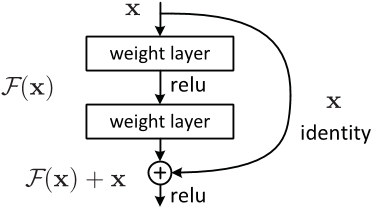
\includegraphics[width=.5\linewidth]{resnet}
	\caption{Model of a 2-layer basic residual unit using the identity projection \cite{hekaming2016} }
	\end{center}
\end{figure}

\subsection{Wide residual networks}
Wide residual networks were proposed by Zagoruyko and Komodakis as an alternative to deep residual networks \cite{zagoruyko2016wide}. The authors widen a network by increasing the number of filters per convolutional layer while decreasing the overall depth in the network, in contrast to the original ResNet architecture which was thin and deep. Properly tuned wide networks have fewer parameters than deep networks, thus requiring less memory to store and less time to train. In this project, we briefly experiment with the effects of trading depth for width with a wide variant of our base architecture.

\subsection{Dropout}
Dropout was introduced by Srivastava et al. as a simple stochastic regularization method \cite{srivastava2014dropout}. Dropout reduces the number of active neurons during training time by setting the output of a neuron to 0 with probability $p$. Intuitively, this forces the next layer in the network to train on sparser and more randomized input, which helps prevent overfitting on the training data. In the original formulation of dropout, zeroing does not occur during inference. Instead, outputs are simply scaled by $(1 - p)$ to their expected values. This requires additional computation during inference time, which is undesirable. As a solution, inverted dropout combines zeroing and scaling output by $1 / (1 - p)$ during training so that no additional computation is required during inference. Our model makes use of periodic inverted dropout for regularization.


\subsection{Softmax cross-entropy loss}
Softmax cross-entropy loss is one of the standard loss function for classification problems. For a single example, given the class score output $s_1, s_2, \dots, s_C$ of a neural network, the scores are converted to probabilities $p_1, \dots, p_C$ via the softmax function $$p_i = \sigma(s_i) = \frac{e^{s_i}}{\sum_{j = 1}^C s_j}$$ Let $y$ be the correct class. Then, the cross-entropy loss is $$L = -\log p_y = -\log \left( \frac{e^{s_y}}{\sum_{j = 1}^C s_j} \right)$$ Cross-entropy loss has the advantage of being differentiable, in contrast with SVM loss which is not. In addition, cross-entropy loss aims to drive all incorrect class scores to 0 while SVM loss is only concerned with increasing the correct class score above a certain margin.

\subsection{Adam optimization}
Adam is an adaptive learning rate optimization algorithm which incorporates both moving average of moments to achieve per-parameter scaling of updates. In particular, it increases the step size of variables with slow moving updates and decreases the step size of fast moving updates. It is similar to the RMSProp optimization, but also incorporates momentum updates. Given learning rate $\alpha$, decay parameters $\beta_1, \beta_2$, and numerical stability constant $\epsilon$, the update step is
\begin{align}
m &:= \beta_1 m + (1 - \beta_1) \nabla x \\
v &:= \beta_2 v + (1 - \beta_2) \nabla x^2 \\
x &:= x - \alpha \frac{m}{\sqrt(v) + \epsilon}
\end{align}

\subsection{Convolutional network architectures}
In this project, we explore four different convolutional network architectures. The basic architecture consists of an initial 7x7 convolutional layer. This layer is then followed by a series of 12 3x3 residual units, for a total of 25 convolutional layers (not including layers used for residual projection). Every third residual unit, the feature map size is halved by increasing stride while the number of filters is doubled. At the end of the network, global average pooling is used and followed by a fully connected layer to output logits for softmax cross-entropy loss. Dropout is applied on the initial input, every third residual unit, and before the fully connected layer.

The wide variant of the architecture replaces the 12 residual units with 8 residual units of doubled width, for a total of 16 convolutional layers. Dimension changes occur every second residual unit rather than every third unit, and dropout is applied every second unit rather than every third. The rest of the architecture remains the same.

The widest variant of the architecture consists of an initial 7x7 convolutional layer followed by 3 wide 3x3 residual units. The residual units are followed by a bottleneck layer then a 2048-filter layer, for a total of 9 convolutional layers. As in the basic architecture, global average pooling and a fully connected layer are used to generate logits. Dropout is applied on the initial input, after residual units, and before the fully connected layer.

The fourth fusion variant is almost identical to the basic architecture, but doubles the width of the last set of 3 residual units to 1024, as a more controlled experiment on the effects of width.

\begin{figure}[h]
\begin{center}
\begin{tabular}{l | r}
Layer & Output Size \\ \hline \hline
Input	& 128x128x1\\
Dropout &  \\
7x7 conv, 64, /2	 & 64x64x64\\
3x3 residual unit, 64	& 64x64x64\\
3x3 residual unit, 64 & \\
3x3 residual unit, 64	& \\
Dropout	&  \\
3x3 residual unit, 128, /2 & 32x32x128\\
3x3 residual unit, 128 & \\
3x3 residual unit, 128 &\\
Dropout & \\
3x3 residual unit, 256, /2 & 16x16x256\\
3x3 residual unit, 256 & \\
3x3 residual unit 256	 & \\
Dropout	& \\
3x3 residual unit, 512, /2	& 8x8x512\\
3x3 residual unit, 512	&\\
3x3 residual unit, 512& \\
8x8 Average Pooling	& 512\\
Dropout& 	\\
Fully connected, 250	& 250
\end{tabular}
\caption{Basic convolutional network architecture.}
\end{center}
\end{figure}

\begin{figure}[h]
\begin{center}
\begin{tabular}{l | r}
Layer & Output Size \\ \hline \hline
Input	& 128x128x1\\
Dropout &  \\
7x7 conv, 128, /2	 & 64x64x128\\
3x3 residual unit, 128	& 64x64x128\\
3x3 residual unit, 128 & \\
Dropout	&  \\
3x3 residual unit, 256, /2 & 32x32x256\\
3x3 residual unit, 256 & \\
Dropout & \\
3x3 residual unit, 512, /2 & 16x16x512\\
3x3 residual unit, 512 & \\
Dropout	& \\
3x3 residual unit, 1024, /2	& 8x8x1024\\
3x3 residual unit, 1024	&\\
8x8 Average Pooling	& 1024\\
Dropout& 	\\
Fully connected, 250 	& 250
\end{tabular}
\caption{Wide convolutional network architecture.}
\end{center}
\end{figure}

\begin{figure}[h]
\begin{center}
\begin{tabular}{l | r}
Layer & Output Size \\ \hline \hline
Input	& 128x128x1\\
Dropout & \\
7x7 conv, 256, /2	 & 64x64x256\\
3x3 residual unit, 256	& 64x64x256\\
Dropout	&  \\
3x3 residual unit, 256, /2 & 32x32x256\\
Dropout & \\
3x3 residual unit, 512, /2 & 16x16x512\\
Dropout	& \\
1x1 conv, 256 & 16x16x256 \\
3x3 conv, 2048, /2 & 8x8x2048 \\
8x8 Average Pooling	& 2048\\
Dropout& 	\\
Fully connected, 250	& 250
\end{tabular}
\caption{Widest convolutional network architecture.}
\end{center}
\end{figure}

\begin{figure}[h]
	\begin{center}
	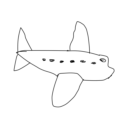
\includegraphics[width=0.5\linewidth]{airplane}
	\caption{Example sketch from TU Berlin dataset.}
	\end{center}
\end{figure}


%-------------------------------------------------------------------------
\section{Approach}
We first preprocess the dataset to produce 128 x 128 px images. The original images are rescaled from 1111 x 1111px to 128 x 128px via bilinear interpolation. The resized images are then read into memory as grayscale 128x128 arrays.

Our approach follows a fairly standard image classification pipeline. Image arrays are fed into a CNN with the final output being fed to a 250-unit fully connected layer to generate logits for each class. We then apply a softmax loss function to the logits and optimize the loss using the Adam algorithm.

We tried to train multiple deep ResNets varying from x to x layers to see which one performs better on the TU-Berlin dataset. The network with the most layers was the one that performed the best showing that ConvNets are able to learn concepts that are more abstract with the depth of the network. This is important to highlight, because sketches are generally very abstract. All of the CNNs were trained with batch size of 32. 


With varying amount of layers to make the model deeper, we also tried several approaches of dropout to counter overfitting as well as different sizes of width for our filters. A more aggressive dropout of 60 and a lesser aggressive dropout of 25 does not improve our validation accuracy.  We also tried a variation of width for our layers. Using these different parameters, our best model was our Vanilla ResNet. This best performing model can be seen in Figure 2. With this model, we were able to achieve a test accuracy of 65.15, but the other types of parameters fall within this range of accuracy. The results are brought in Table 1. Note: all of our models are trained for the same number of epochs. 

\begin{table}[h]
\begin{center}
\begin{tabular}{|l|c|}
\hline
Method & \% \\
\hline\hline
ResNet-aggro-dropout &  65.3 \\
ResNet Vanilla & 65.15 \\
ResNet Weak Dropout & 65.6\\
ResNet Wide &  65.3\\ 
ResNet  Wide V2 & 63.9\\
ResNet Wider  &  58.8\\
ResNet Widish  & 62.05\\ 
ResNet Widest &  55.8\\
\hline
\end{tabular}
\end{center}
\caption{Validation performance comparison between our different parameters}
\end{table}

In Table 1 and Figure 7, we compared all of our model's training and validation accuracies. Looking at the training accuaries (Figure 7), we see that there is a rapid increasement of accuracy over the amount of epochs. The Vanilla ResNet architecture increases most rapidly compared to the others models, but the ResNet-Weak-dropout model reaches the same training accuracies as the Vanilla ResNet model. The Canilla ResNet and Weak-dropout ResNet architecture have the highest training accuracy compared to the other models. On the other hand, all our validation accuracies level out near the end of training. There is a drastic drop in the validation accuracy for Widish-ResNet model, but it the accuracy picks back up and ends up within the same range of validation accuracies as the other models. 

The difference between training accuracy and validation accuracy of our models is a good indicator of overfitting. Based on our results, we realized that ResNets are more prone to overfitting. However, these results show that adding a simple shortcut connection can improve the accuracy in the classification task and make the training process much faster, but  the trade of is that residual networks are more prone to over-fitting which is undesirable. Our results also suggest that depth is the largest contributing factor to classification accuracy, with dropout regularization providing minor improvement. Widening layers does not result in noticeable changes, and the need to reduce memory consumption by reducing network depth in fact leads to lower accuracy. 
>>>>>>> Stashed changes

\begin{table}[h]
\begin{center}
\begin{tabular}{|l|c|}
\hline
Method & \% \\
\hline\hline
SIFT-varient + BoF + SVM  ~\cite{eitz2012hdhso}  &  56 \\
IDM + SVM ~\cite{yesilbek2015svm} & 71.30 \\
ConvNet ~\cite{seddati2015deepsketch}  & 75.42\\
ConvNet ~\cite{seddati2016deepsketch} & 77.69\\
ConvNet --Ours & 0.4 \\
\hline
\end{tabular}
\end{center}
\caption{Test accuracy comparison of our models versus other methods.}
\end{table}

Our experiments illustrate the complexity of free-hand sketch recognition. An example of the variability of sketches can be seen in Figure 5. This type of varaibility of sketches causes the model to be confused. Where if some edges are similar to another previous trained edge, it will think that particular sketch will belong to a class that is not its true class. An example of such can be viewed in Figure 6. For Figure 6, the model was presented with the airplane (right), and the model classified it as a syringe (left). Notice how similar the edges are within these two sketches, and there is no "true" airplane wing either which is a distinguishable feature for an airplane. 

Table 2 summarizes the overall performance in terms of average recognition accuracy for various architectures compared to our highest performing model. While our CNN  model?s performance is not quite as strong as the CNN model of [~\cite{krizhevsky2012imagenet}], in terms of test accuracies, we would like to point out that the authors used a larger CNN on a larger external dataset through pooling additional sketches through Google. 



\begin{figure}[h]
	\begin{center}
	\includegraphics[width=1\linewidth]{Spondgebob}
	\caption{ Examples of interclass variations of Spongebob from the TU Berlin dataset highlighting the variability }
	\end{center}
\end{figure}


Though our model was able to outperform the traditional multi-class support vector classifiers (SVMs) [1] , there is still more improvement that can be done. Along with that, we were not able to train the model as long as we would have hoped. If you notice in Figure 7 the validation accuracy for our models has not completely leveled out. An example of an error our model made can be seen in Figure 5. 


%-------------------------------------------------------------------------
\section{Experiments}
Our current model consists of three convolution-batch normalization-ReLU-max pooling layers, followed by a fully connected layer to output logits. Loss is computed as softmax cross entropy. With this model, we were able to achieve a test accuracy of 0.004, which is the same as random guessing, so there is still work to be done.

\begin{figure}[h]
\begin{center}
\begin{tabular}{l | l | l}
Layer & Output Size & Feature Depth \\ \hline \hline
Conv-7 & 128x128 & 32 \\
BN & 128x128 & 32 \\
ReLU & 128x128 & 32 \\
MaxPool-2, /2 & 64x64 & 32 \\ 
Conv-5 & 64x64 & 64 \\
BN & 64x64 & 64 \\
ReLU & 64x64 & 64 \\
MaxPool-2, /2 & 32x32 & 64 \\ 
Conv-3 & 32x32 & 128 \\
BN & 32x32 & 128 \\
ReLU & 32x32 & 128 \\
MaxPool-2, /2 & 16x16 & 128 \\
FC & 250 &
\end{tabular}
\caption{ConvNet architecture. The "-$f$" notation refers to a layer with a $f$x$f$ filter. The "/$s$" notation refers to a layer with stride $s$.}
\end{center}
\end{figure}

%-------------------------------------------------------------------------
\section{Conclusion}

In this paper, we have presented our CNN architecture for freehand sketch recognition. We see that in our model, where free-hand sketches are inherently hard to classify due to large amounts of intraclass variation and interclass overlap, along with a lack of complex visual information, in contrast to traditional image recognition which instead deals with an overabundance of visual information. 
Sketches are usually centered around the edges, and for most neural networks edge detection is within the first few layers. 

Our experiments showed that moderate dropout with deep networks provides the best results. Overaggressive dropout and shallow networks both lead to lower accuracy. Notably, compensating for shallowness with increased width does not result in improved accuracy. 
ResNets are more powerful for very deep networks and and can hurt the performance for shallow networks. ResNets, however, does show promising landscape in deep learning. 

The TU-Berlin dataset, though is the largest, is still relatively limited. However, some things that we can try next is use other networks to train on the TU- Berlin dataset, such as using VGG to train on sketches or the original architecture of ResNet. Our framework source-code and associated data (pre-trained models) can be accessed at: github.com/krinkels/sketch-recognition

{\small
\bibliographystyle{ieee}
\bibliography{milestone}
}

\end{document}
